\begin{flushright} {\tiny {\color{gray} (tikz\_P3.tex)}} \end{flushright}
%~~~~~~~~~~~~~~~~~~~~~~~~~~~~~~~~~~~~~~~~~~~~~~~~~~~~~~~~~~~~~~~~~~~~~~~~~~~~~~~~~~~~~~~~~~~~~~~~~~

\begin{center}
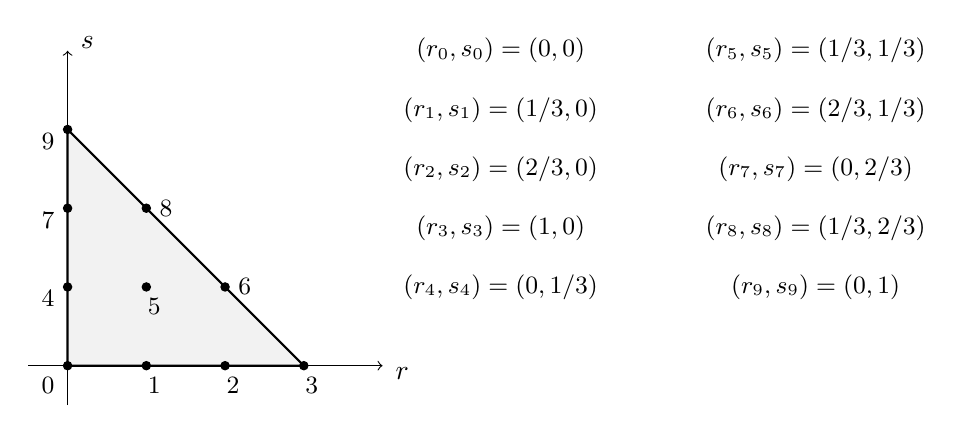
\begin{tikzpicture}
%\draw[step=0.5cm,gray,very thin] (0,0) grid (13,6); 
\draw[fill=gray!10,gray!10] (0.5,0.5)--(3.5,0.5)--(0.5,3.5)--cycle;
\draw[thick] (0.5,0.5)--(3.5,0.5)--(0.5,3.5)--cycle;
\draw [->] (0,0.5) -- (4.5,0.5);
\draw [->] (0.5,0) -- (0.5,4.5);
\node[] at (4.75,0.4) {$r$};
\node[] at (0.75,4.6) {$s$};
\draw[black,fill=black] (0.5,0.5)   circle (1.5pt);
\draw[black,fill=black] (1.5,0.5)   circle (1.5pt);
\draw[black,fill=black] (2.5,0.5)   circle (1.5pt);
\draw[black,fill=black] (3.5,0.5)   circle (1.5pt);
\draw[black,fill=black] (0.5,1.5)   circle (1.5pt);
\draw[black,fill=black] (1.5,1.5)   circle (1.5pt);
\draw[black,fill=black] (2.5,1.5)   circle (1.5pt);
\draw[black,fill=black] (0.5,2.5)   circle (1.5pt);
\draw[black,fill=black] (1.5,2.5)   circle (1.5pt);
\draw[black,fill=black] (0.5,3.5)   circle (1.5pt);

\node[] at (0.25,0.25) {\small $0$};
\node[] at (1.6,0.25)  {\small $1$};
\node[] at (2.6,0.25)  {\small $2$};
\node[] at (3.6,0.25)  {\small $3$};
\node[] at (0.25,1.35) {\small $4$};
\node[] at (1.6,1.25)  {\small $5$};
\node[] at (2.75,1.5)  {\small $6$};
\node[] at (0.25,2.35) {\small $7$};
\node[] at (1.75,2.5)  {\small $8$};
\node[] at (0.25,3.35)  {\small $9$};

\node[] at (6,4.5)  {\small $(r_0,s_0)=(0,0)$};
\node[] at (6,3.75) {\small $(r_1,s_1)=(1/3,0)$};
\node[] at (6,3)    {\small $(r_2,s_2)=(2/3,0)$};
\node[] at (6,2.25) {\small $(r_3,s_3)=(1,0)$};
\node[] at (6,1.5)  {\small $(r_4,s_4)=(0,1/3)$};

\node[] at (10,4.5)  {\small $(r_5,s_5)=(1/3,1/3)$};
\node[] at (10,3.75) {\small $(r_6,s_6)=(2/3,1/3)$};
\node[] at (10,3)    {\small $(r_7,s_7)=(0,2/3)$};
\node[] at (10,2.25) {\small $(r_8,s_8)=(1/3,2/3)$};
\node[] at (10,1.5)  {\small $(r_9,s_9)=(0,1)$};


\end{tikzpicture}
\end{center}

